\documentclass[11pt]{article}

\usepackage{amsmath}
\usepackage{float}
\usepackage{graphicx}
\usepackage{subcaption}

\begin{document}
    \title{HPCSE II - Exercise 2}
    \author{Anian Ruoss}
    \maketitle

    \subsection*{Task 4}

    \begin{figure}[H]
        \begin{subfigure}{.5\textwidth}
            \begin{center}
                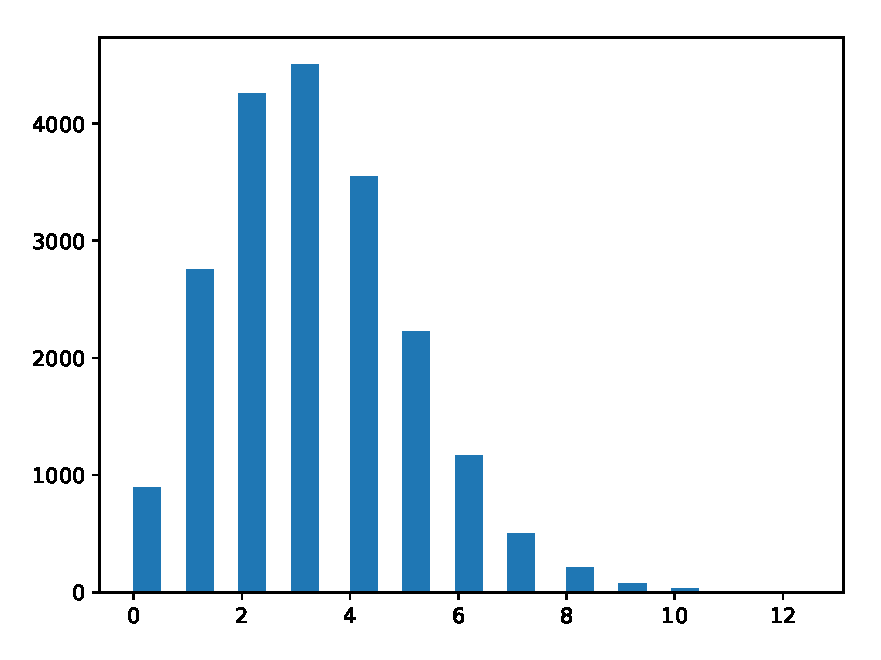
\includegraphics[width=\textwidth]{plots/hist.eps}
                \caption{Unnormalized}
            \end{center}
        \end{subfigure}
        \begin{subfigure}{.5\textwidth}
            \begin{center}
                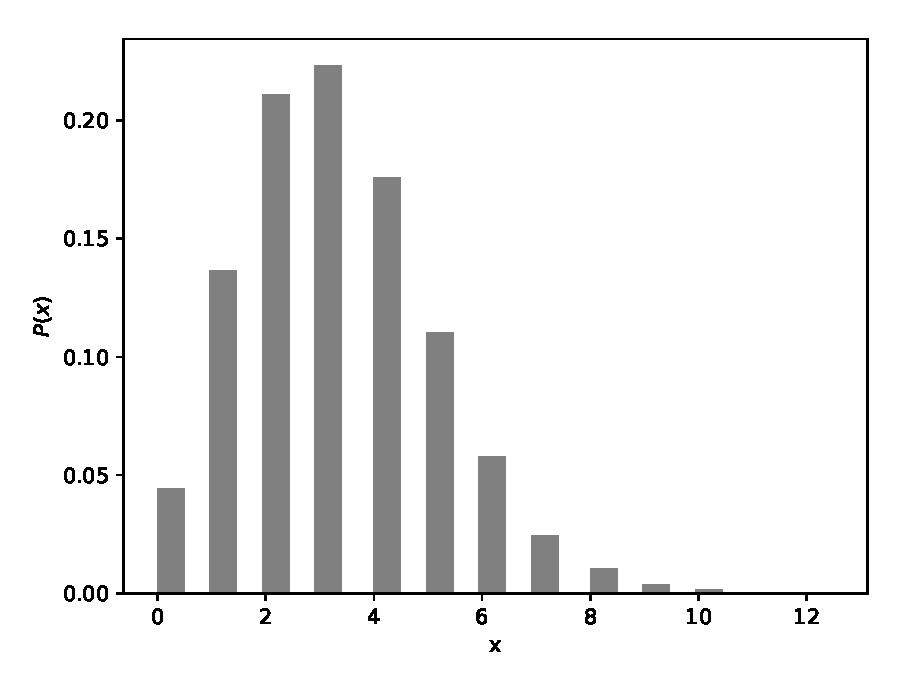
\includegraphics[width=\textwidth]{plots/hist_normalized.eps}
                \caption{Normalized}
            \end{center}
        \end{subfigure}
        \caption{Histogram of data with 100 bins.}
    \end{figure}

    \begin{figure}[H]
        \begin{center}
            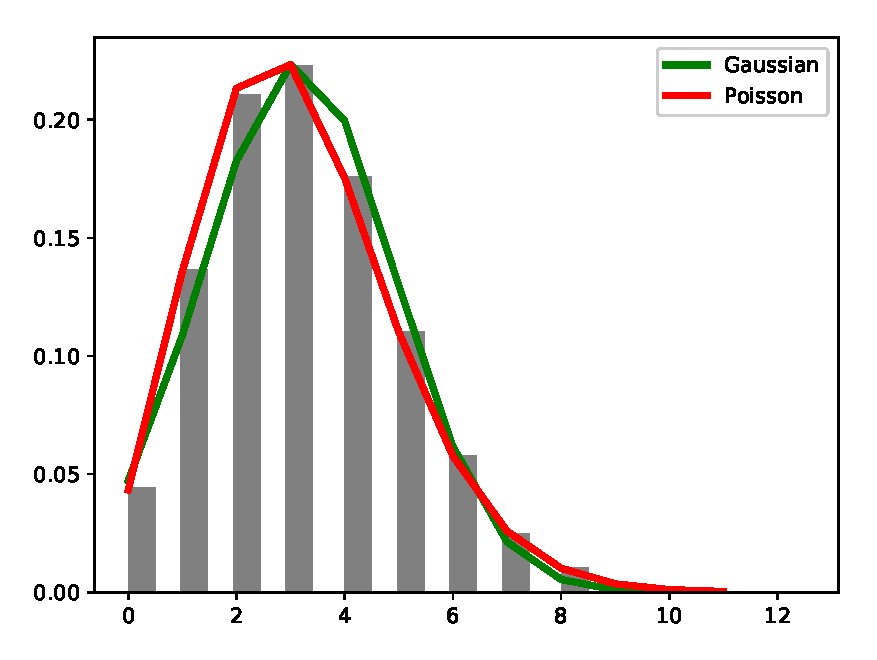
\includegraphics[width=.5\textwidth]{plots/hist_distributions.eps}
        \end{center}
        \caption{Normalized histogram and distributions from MLE parameters.}
    \end{figure}

\end{document}